Afin de permettre une meilleure gestion du projet (travail parallèle, gestion de bugs, etc.) nous avons décidé d'utiliser le gestionnaire de version Git ainsi que la forge GitLab mise à la disposition des étudiants par le SIF.
La prise en main fut facile, les membres du groupe ayant pratiquement tous déjà utilisé cet outil. Nous avons également utilisé le système de suivi de bugs intégré à Gitlab (cf. Figure~\ref{bugs}).
\begin{figure}[h]
\centering
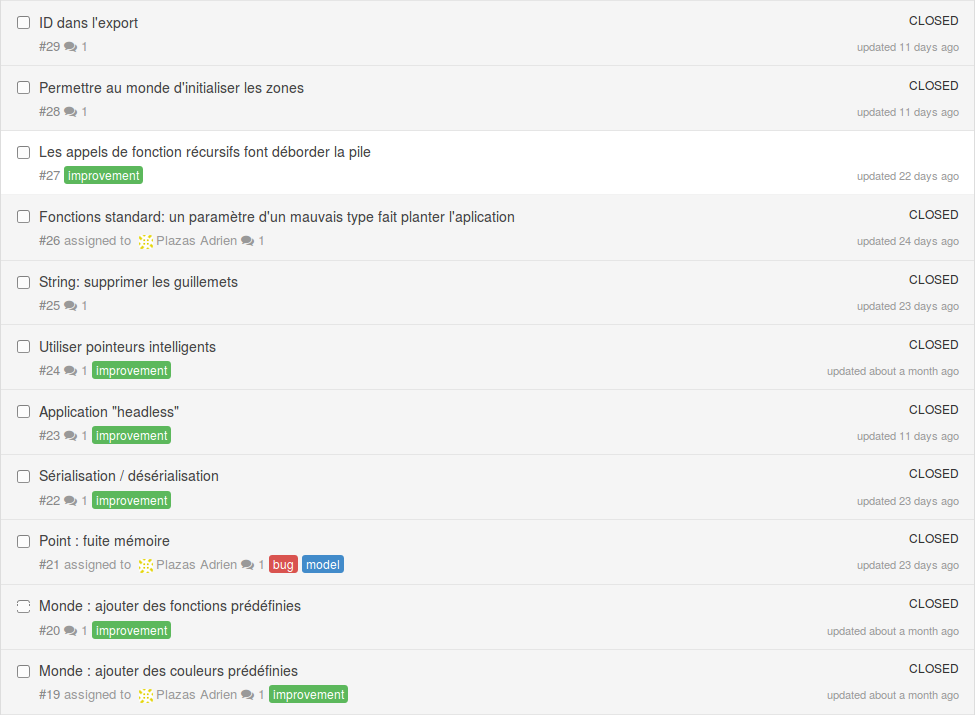
\includegraphics[scale=0.35]{doc/gestionProjet/bugs.png}
\caption{\label{bugs} Système de suivi de bugs de Gitlab}
\end{figure}

Notre organisation des branches fut la suivante~:
\begin{itemize}
\item la branche master devait contenir une version fontionnelle compilable~;
\item des branches de développement étaient créées pour chaque nouvelle fonctionnalité, et n'étaient fusionnées sur la branche master que lorsqu'elles étaient pleinement fonctionnelles~;
\item des branches spécifiques à chaque version ont été dérivées de master lors de l'officialisation desdites versions.
\end{itemize}

Nous utilisions également Gitg, pour avoir une meilleure vue de l'état de notre dépôt (cf. Figure~\ref{Gitg}).

\begin{figure}[h]
\centering
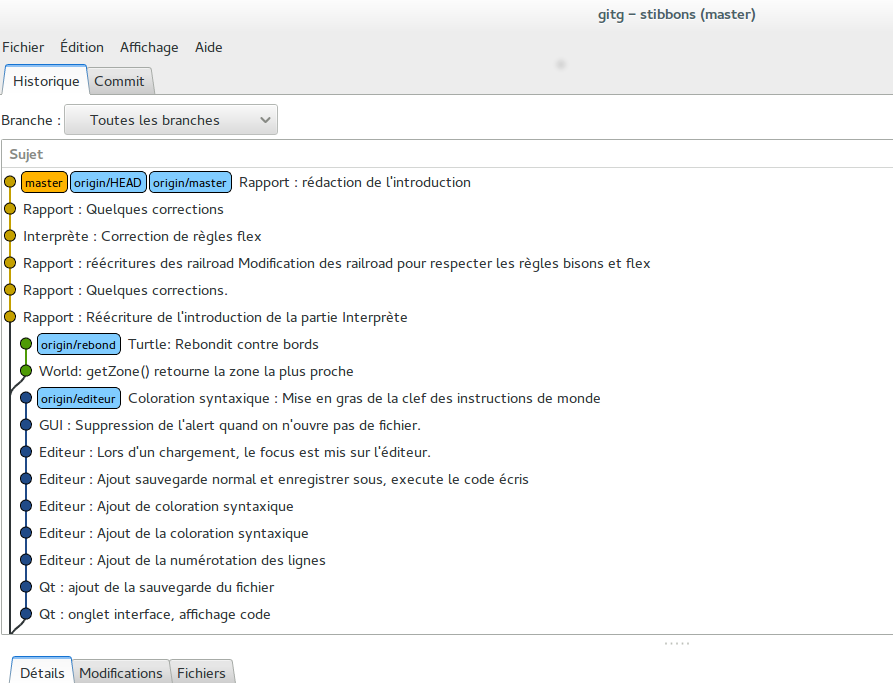
\includegraphics[scale=0.35]{doc/gestionProjet/gitbranche.png}
\caption{\label{Gitg} Vue des branches dans Gitg}
\end{figure}
